\begin{wordonframe}{Mordasini18 MAIN RESULTS}
\begin{itemize}
\item Cosa ho messo nel modello e2e? (Montecarlo variables) Disk metallicity $[M/H]$ (Santos 05) and $f_{dg}$ (Lodders 03). Initial disk mass: stability (SHu 90), observation (andrws 10, manara 16) MMSN; Disk lifetime (Haisch 01, mamajek 09); starting embryos position
planetesimal size is 300m, planetesimal distro $\propto r\expy{-1.5}$ and outer exponential radius half that of gas to account inward drift (kornet 01; birnstiel andrews 14) and more concentrated distro resulting from planetesimal formation (drazkowska 16) - ''The TW Hya Disk at \SI{870}{\micro\meter}:  Comparison of CO and Dust Radial Structures'' 2011; planetesimal size 300m: what's influenced?
Struttura disco accrescimento: calibrazione tempo di vita, evoluzione viscosa ed evaporazione - $\alpha=0.002$.
Evoluzione embrioni: accrescimento, evoluzione orbitale (N-body+migration timescale+e,i damping)

\item Distribuzione massa pianeti: distribuzione bimodale con discrimine a $30\mearth{}$.
\begin{figure}[!ht]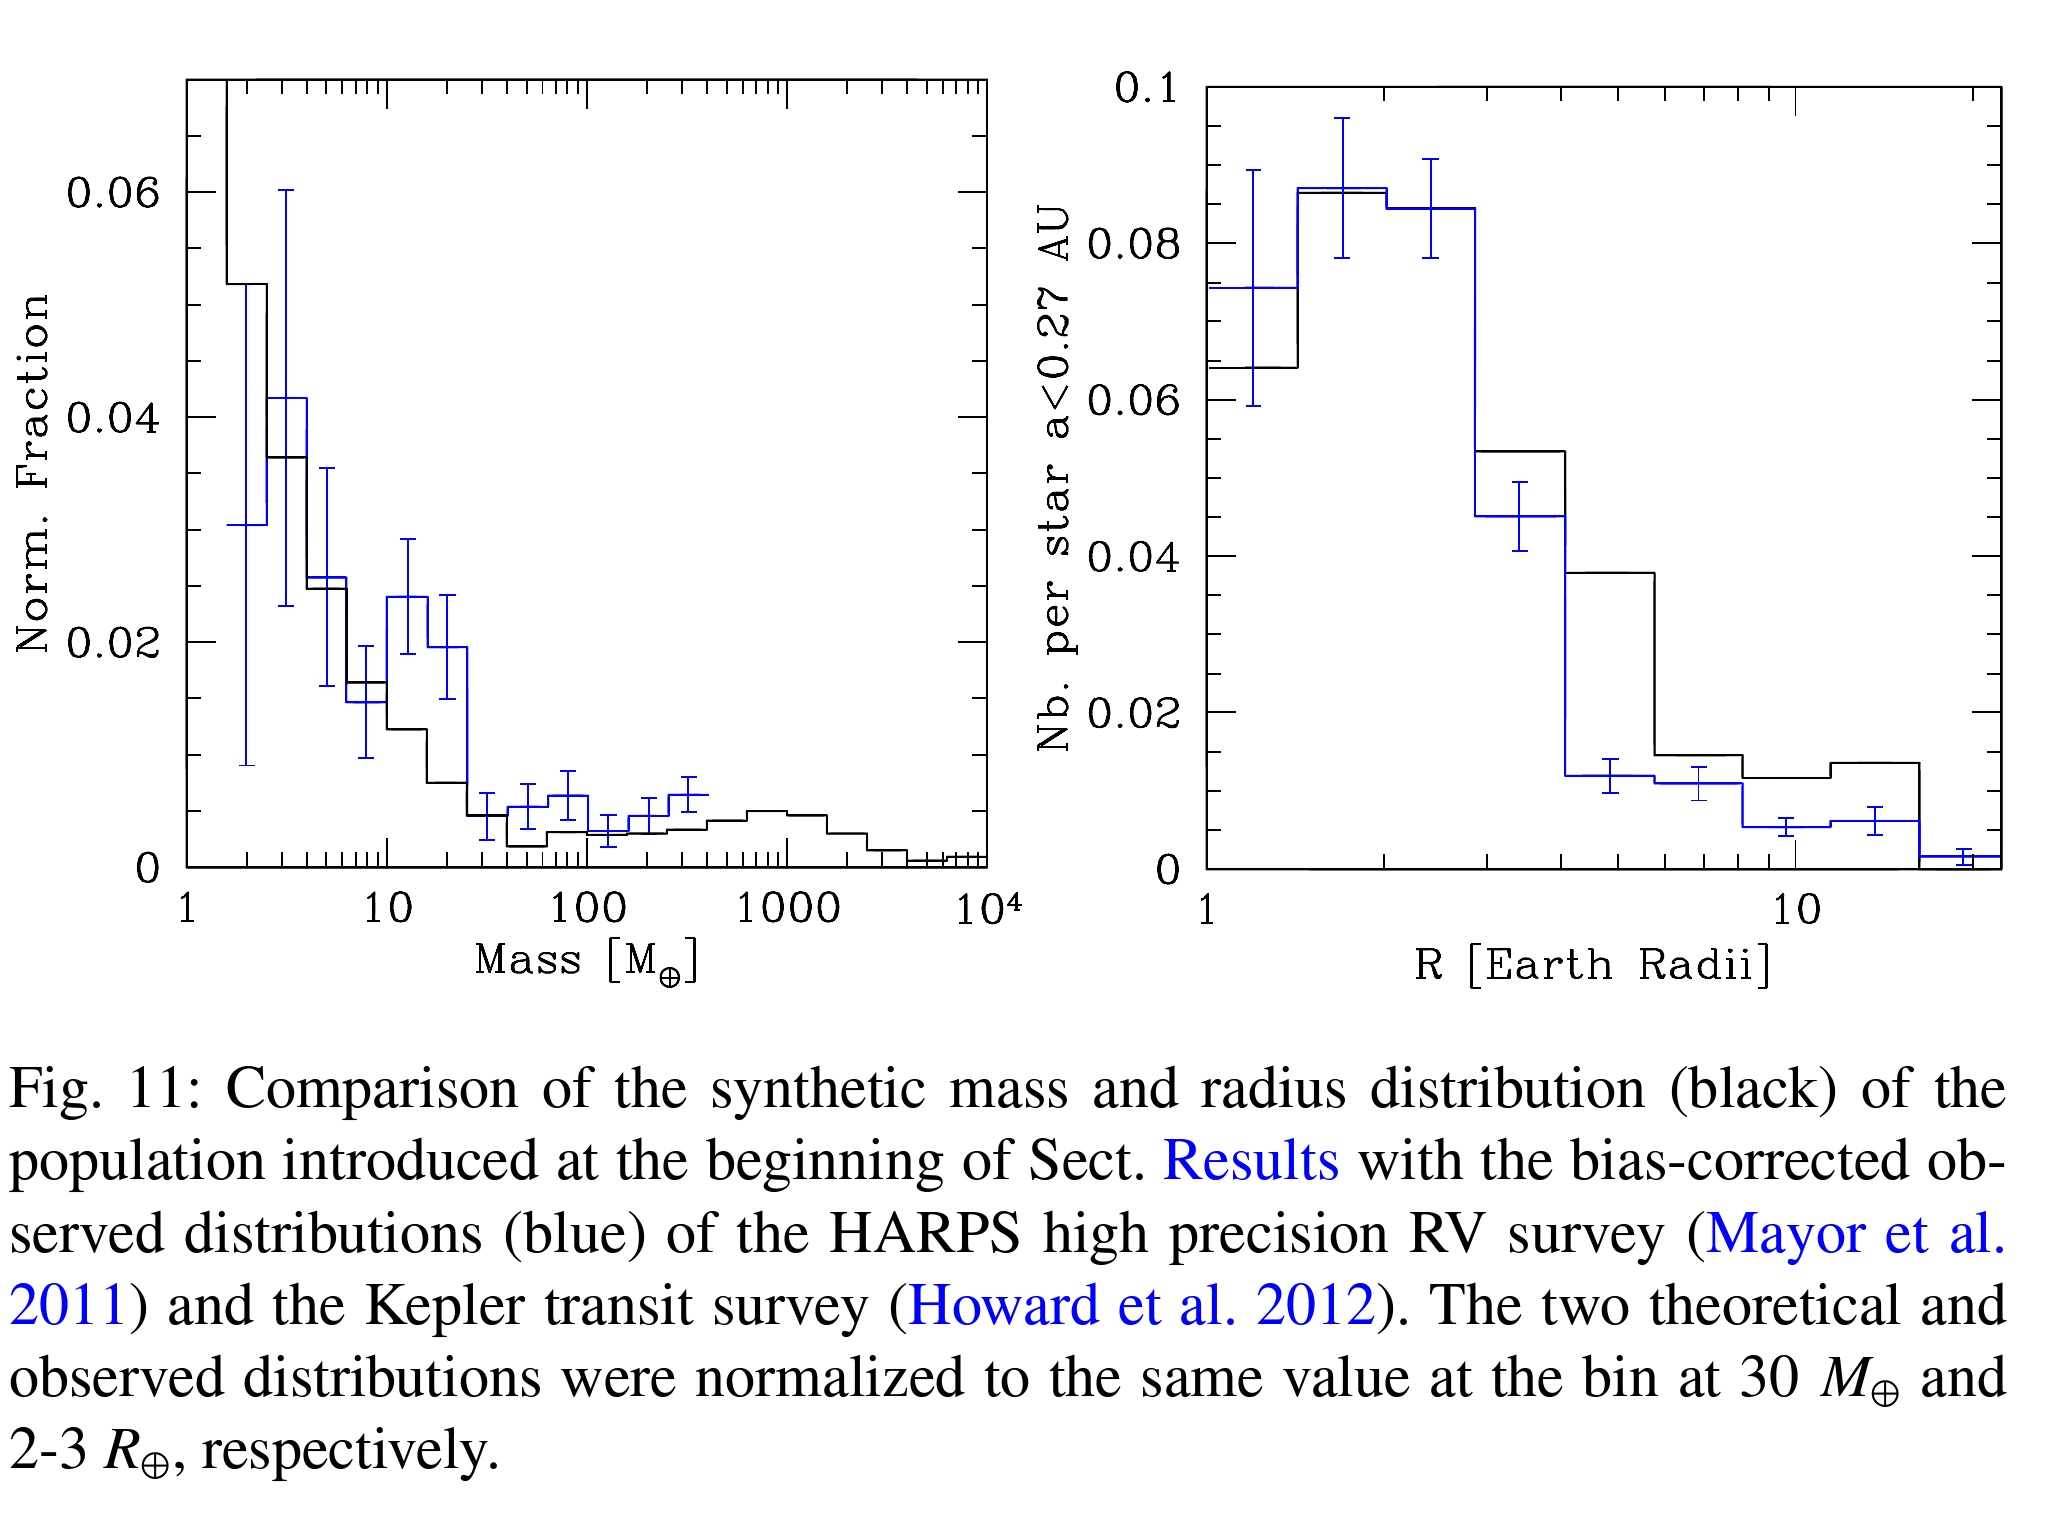
\includegraphics[trim={0cm 17cm 0 0},clip, keepaspectratio,width=0.9\textwidth]{MR-freq-obssynth}\caption{Distribuzioni di massa e raggio per popolazione planetaria sintetica (linea nera) e distribuzioni osservate tramite RV e transiti (linea blu) corrette per i bias. Da \cite{mordasini2018planetary}.}\label{fig:MR-freq-obssynth}\end{figure}
Massa critica per accrescimento di gas: tempo scala accrescimento planetesimi vs tempo scala disco.
Tempi scala migrazione
\item distribuzione in semiassi che dipende da posizione iniziale embrione: necessity to include earlier planetary formation; montecarlo variable: initial starting position embryos- kokubo ida 00: uniform distro in log(a) (vedi anche ida lin 10) (dov'era scritto del comportamento caotico??+); hasegawa pudritz 11, cridland 16: embryos rapidly moves into traps.
Preferred formation regions of planetesimal (Drazkowska16; brauer 08), particle pile-up outside orbits of already existing planets (Pinilla15), strong migration traps (Horn 12, Hasegawa Pudritz 12).
Disc/planetesimals parameters: planetesimal has steeper profile $\propto r\expy{-3/2}$, outer exponential radius half that of gas: inward drift of dust (kornet 01, birnstiel Andrews 14), concentrated distro resulting from planetesimal formation (Drazkowska 16);
\item Distribuzione raggi: diagramma massa-raggio, composizione, evaporazione.
\item (Mordasini pg 27) LArge majority are low mass planets ($0.1-10\mearth{}$), 
\item frequency of giant, close-in and habitable planets. The high frequency of close-in planets can be reproduced assuming steep distribution of planetesimal and centrally concentrated (chiang laughlin 13, drazkowska 16)
\item correlation with disk properties (mordasini 12a): metallicity effects (mortier13)
\item Sub-saturn mass desert (ida lin 04) not seen in kepler data (Thompson 18): accretion of planetesimal slow down gas accretion
\item migrazione, cattura risonante: ''On the migration of two planets in a disc and the formation of mean motion resonances'' Migaszewski 15; ''Perturbation of compact planetary systems by distant giant planets'' Hansen 17
\end{itemize}
\end{wordonframe}